\documentclass[11pt]{article}
\usepackage[margin=1in]{geometry}
\usepackage[T1]{fontenc}
\usepackage{amsmath,amssymb}
\usepackage{booktabs,tabularx,array}
\usepackage{graphicx}
\usepackage{tikz}
\usepackage[hidelinks]{hyperref}
\usepackage{listings}
\setlength{\parindent}{0pt}
\setlength{\parskip}{0.55\baselineskip}
\lstset{basicstyle=\ttfamily\small,breaklines=true,columns=fullflexible,frame=single}

\title{Is AI ``Slop'' Taking Over the Internet?\\
\large Evidence, a Measurement Protocol, and an Interpretable Detection Baseline}
\author{Research draft}
\date{September 10, 2026}

\begin{document}
\maketitle

\begin{abstract}
Low-quality AI-generated text raises two questions that are often conflated:
how much of it is being published, and how reliably it can be recognized.
This project examines both without assuming that an internet-wide takeover
has occurred. We distinguish growth in machine-written content from poor
quality and from dominance of a particular web population or audience's
exposure. A review of existing evidence informs a longitudinal sampling
protocol and a transparent detector with separate authorship and quality
classifiers. The code supports training, validation-based threshold selection,
held-out evaluation, and feature-level explanations. A small authorship pilot
now pairs 12 historical magazine articles with 12 assistant-generated articles.
All eight candidate settings achieve perfect validation ranking and recall,
yet the selected model detects none of the three generated test articles at
its frozen threshold. That failure illustrates why a favorable ranking metric
cannot stand in for a useful decision rule. The broader prevalence study and
independently annotated quality evaluation remain unfinished; the pilot is
not evidence of modern-web accuracy or an internet-wide takeover. A second
exploratory cycle now reuses all pilot articles as development material,
examines threshold stability and feature controls, and freezes a prospective
methodology. Contemporary corpus acquisition, independent human annotation,
and a new untouched evaluation remain outstanding.
\end{abstract}

\section{Introduction and Research Questions}
Cheap automated publishing could crowd out useful human communication. That
concern is the starting point, not the finding. ``AI-generated,'' ``low
quality,'' and ``taking over'' describe different things: a carefully checked
AI-assisted tutorial can be useful, just as a human-written article can be
misleading. Treating origin as a verdict on quality would build the desired
answer into the definition. We instead measure the two separately.

The study concerns \emph{English-language public-web text}, with a deliberately
limited scope that makes the proposed measurements reproducible. Images,
audio, video, private messages, and bot traffic are outside the first study.
Four questions guide the investigation:
\begin{enumerate}
\item \textbf{RQ1---Prevalence:} Has the proportion of AI-generated or
AI-assisted text increased within a clearly defined web sampling frame?
\item \textbf{RQ2---Quality:} What proportion of that content meets an
independently defined low-quality rubric?
\item \textbf{RQ3---Detection:} Can a transparent model identify the intersection
of machine authorship and low quality while limiting false accusations?
\item \textbf{RQ4---Generalization:} How does detection change for unfamiliar
publishers, generators, genres, and edited text?
\end{enumerate}

\textbf{Claim discipline.} ``Proving it'' should mean testing a falsifiable
hypothesis, not collecting a gallery of alarming examples. Growth does not
establish a majority. Nor would a majority of newly published pages establish
a majority of all existing pages, much less of the material people actually
see. A study that finds the takeover hypothesis unsupported can still succeed
as research.

Consider a publisher that places many near-identical pages online but attracts
few readers. Those pages count toward a publication-based measure, although
their contribution to exposure may be small. Conversely, one heavily visited
page may account for considerable exposure without noticeably changing the
page count. These are hypothetical cases, but they clarify the measurement
problem: the unit being counted must be chosen before the result is interpreted.
The paper therefore asks what a denominator represents before asking whether
a reported percentage is large.

\section{Existing Evidence: What Is Established?}
\subsection{Growth depends on the denominator}
In its August 20, 2026 analysis, Pew Research Center reports signs of AI
authorship in approximately 10\% of an English-language webpage snapshot from
July 2026. The share rises to approximately 35\% among pages with publication
dates after ChatGPT's release \cite{pew}. Both figures are detector-based
estimates. Neither represents verified authorship or the prevalence of
low-quality content.

The analysis sampled 10,000 pages from each of 49 Common Crawl snapshots
between January 2021 and July 2026. Publication dates could be extracted for
only about 10--15\% of the pages, so the dated subset was not random. Material
behind logins or paywalls was also underrepresented \cite{pewmethods}. The
dated-page estimate consequently describes a narrower population than the
internet as a whole.

Dolezal and colleagues reach a related estimate in an April 2026 preprint:
roughly 35\% of newly published websites in their Internet Archive sample were
classified as AI-generated or AI-assisted by mid-2025. They find associations
with reduced semantic diversity and increased positive sentiment, but no
statistically significant support for declining factual accuracy or stylistic
diversity \cite{dolezal}. The null findings do not establish that harm is
absent. They do mean that these hypothesized harms cannot all be presented
as observed outcomes.

\subsection{Detection is not ground truth}
RAID contains more than six million generations across 11 models, eight
domains, 11 adversarial attacks, and four decoding strategies. Its evaluations
expose weaknesses when generators, decoding choices, or adversarial
transformations change \cite{raid}. Tufts and colleagues find similarly
limited recall at a 1\% false-positive operating point, including zero recall
in some settings \cite{tufts}. A detector's reported performance therefore
needs a dataset, a set of model families, and an operating threshold attached
to it. Without them, a headline accuracy is difficult to interpret.

Several detectors evaluated by Liang and colleagues disproportionately
misclassified non-native English writing; prompting also helped generated
text evade detection \cite{liang}. For this project, differences in
false-positive rates are therefore part of the evaluation itself, not an
optional qualification to an overall accuracy score.

\textbf{Evidence-based conclusion.} The studies motivate an investigation of
the growing machine-written component in sampled web text. They do not show
that most internet content is low-quality AI output. We interpret them as
evidence that prevalence, quality, and exposure need separate measurements,
and do not pool their percentages: the populations and operational definitions
differ \cite{pew,pewmethods,dolezal}.

\section{Operational Definition of AI ``Slop''}
For this study, let $A_i=1$ denote documented fully machine-generated origin
and $Q_i=1$ denote independently annotated low quality. Define the primary
binary target as
\begin{equation}
 S_i = A_i Q_i.
\end{equation}
The definition gives an informal term a testable meaning within this study;
it does not assert a universal scientific meaning for ``slop.'' We record
mixed human--AI authorship separately rather than forcing it into either
origin class. A secondary analysis may include substantial AI assistance in
$A_i$, provided that the broader definition is stated explicitly.

Quality assessors, blinded to origin and detector scores, rate three dimensions
from 0 (no material defect), through 1 (noticeable but limited defect), to
2 (substantial defect):
\begin{enumerate}
\item \textbf{Factual and evidential adequacy:} central claims contradict
checkable evidence, or important asserted evidence cannot be substantiated.
\item \textbf{Information value:} substantial redundancy or generic padding
without answering the stated question or adding relevant information.
\item \textbf{Relevance and coherence:} major contradictions, irrelevant passages,
or failure to serve the document's apparent purpose.
\end{enumerate}
Under the initial rule, $Q_i=1$ when at least two dimensions score 2, or when
a verified central factual error defeats the document's purpose. The rubric
must respect genre. Invented events are not a defect in fiction, and a
personal narrative need not supply scholarly citations. Cases that cannot be
resolved receive an uncertain label; they are excluded from binary training,
but their frequency is reported. An isolated document cannot, under this
rubric, establish either malicious intent or mass production.

Two annotators independently label each evaluation document, and a third
resolves disagreements. The analysis reports raw agreement, Cohen's kappa
for the binary quality decision, and disagreement on each dimension. A
separate pilot establishes the rubric before it is frozen for test annotation.
All four origin-by-quality combinations belong in the corpus; otherwise the
model can learn the invalid shortcut ``machine-generated means bad.''

The annotation record should also preserve the reason for each substantial
defect. An unsupported central claim, for example, should be linked to the
passage in question and the evidence used to assess it. This makes a
disagreement reviewable rather than merely countable. It also distinguishes
two sources of difficulty: annotators may apply the same rule differently,
or they may lack enough evidence to apply it at all. More confident scoring
cannot solve the second problem. Uncertain labels should remain uncertain
until the underlying evidence changes.

\section{Study Design: Testing the Takeover Hypothesis}
\subsection{Two distinct datasets}
\textbf{Prevalence corpus.} The initial collection target is 4,000 documents:
1,000 eligible English-language pages from each of four prespecified annual
archive windows in 2022--2025. Fix the exact crawl identifiers and random seed
before inspecting detector scores. Sample across news, informational blogs,
commercial pages, and discussion pages where the archive permits this
classification. Record selection probabilities, extraction failures, language,
genre, publisher, crawl timestamp, and any independently supported publication
date. Crawl date is not necessarily publication date. Sampling equal genre
counts requires design weights for population estimates.

The population consists of eligible pages in the selected snapshots, not all
internet activity. An exclusion flow diagram should show what was lost at
each preparation step, including the fraction removed by the baseline's
80-token minimum. Repetitive pages must not be excluded merely because they
look like slop; doing so would remove part of the outcome being measured.
Repeated archive captures of one page also need to be distinguished from
separate published copies. Deduplicated content prevalence and page-level
prevalence answer different questions.

\textbf{Detector corpus.} A separate target of 2,400 documents provides for
approximately 600 examples in each origin-by-quality cell, with verifiable
provenance and adjudicated quality. These numbers are collection targets,
not achieved sample sizes or a power analysis. Human writing should come
from consented authors with draft histories or suitably documented archives.
Generated examples need a model identifier, generation date, prompt, and
settings. Multiple generator families and matched topics are required; making
every machine example verbose and every human example concise would create
a trivial substitute task. Unknown-origin pages do not belong in supervised
origin labels. A detector's guess is not provenance.

Before scaling collection, a small pilot can check whether the data interface,
split logic, and decision thresholds work together. The pilot reported below
serves that purpose. It does not replace either of the proposed corpora, and
its readily documented historical sources introduce a serious trade-off:
origin is easier to establish, but the language is less representative of
contemporary web writing.

\subsection{Leakage control and evaluation splits}
The full study assigns approximately 60\% of provenance-corpus clusters to
training, 20\% to validation, and 20\% to testing. Related publishers, authors,
source documents, prompt variants, and near duplicates are joined into
clusters, with every connected cluster kept in one split. If the result is
a giant cluster or a split missing a class, collection must be redesigned
rather than separation weakened. The code checks supplied group IDs and
rejects normalized exact duplicates. It cannot discover all related texts
or determine whether the grouping was done correctly.

A frozen future-time and unseen-generator challenge set tests a different
kind of transfer. Separate sets should cover paraphrased, translated,
mixed-authorship, and short text, with provenance established by documented
labels rather than stylistic impressions. Training on fully generated text
does not, by itself, establish an ability to detect editing assistance.

This separation also governs iterative improvement. Training data estimate
coefficients; validation data guide choices among prespecified candidates.
Once test results have been inspected, they may inform a future development
cycle, but that cycle needs a fresh final test set. Repeatedly changing a
threshold until it looks good on the same test articles would make those
articles part of development, whatever their filename says.

\subsection{Estimands and uncertainty}
For a time window $t$, estimate separate proportions $p_A(t)$, $p_Q(t)$, and
$p_S(t)$. Using audited labels and design weights $w_i$, the slop estimator is
\begin{equation}
 \widehat p_S(t)=\frac{\sum_{i\in t}w_i S_i}{\sum_{i\in t}w_i}.
\end{equation}
For unknown-origin web content, $S_i$ is not directly observed. Report the
detector-positive fraction as such, and use independently labeled, matched
audits to characterize errors. For a fixed binary screen with observed
positive fraction $q$, sensitivity $r$, and false-positive rate $f$,
\begin{equation}
 q = r p + f(1-p),\qquad
 \widehat p = \frac{q-f}{r-f}.
 \label{eq:correction}
\end{equation}
Conditioning on the true binary class gives this identity. Applying it is
harder: the error rates must be representative and must transfer to the
population being measured. For slop prevalence, $r$ and $f$ describe the
\emph{joint screen}, not the authorship classifier alone. When $r$ approaches
$f$, the correction becomes unstable. Estimates outside the unit interval
indicate incompatibility or sampling error; clipping them silently would
conceal the problem rather than resolve it.

The planned analysis uses 2,000 publisher-cluster bootstrap replicates within
sampling strata, propagating uncertainty in both prevalence and audit error
rates. Report sensitivity analyses when unknown authorship prevents reliable
audits. Prespecify the primary contrast
$\Delta=p_S(2025)-p_S(2022)$. Evidence for growth requires a positive lower
95\% confidence bound for $\Delta$. A page-majority interpretation of
``taking over'' requires the lower bound for $p_S(2025)$ to exceed 0.5 in the
defined population. Neither finding establishes causation. Exposure dominance
would require a separate impressions- or traffic-weighted dataset.

\section{Detection Model and How the Code Works}
\subsection{Transparent features}
The implemented baseline, \texttt{detector.py}, converts each document into
ten numerical features: log token count; unique-token fraction; mean token
length; mean sentence length; sentence-length coefficient of variation;
repeated-trigram fraction; repeated-sentence fraction; fraction of tokens
containing digits; URL count per token; and selected punctuation count per
token. Tokens are Unicode word sequences with optional internal apostrophes;
sentence boundaries are approximated by periods, question marks, and
exclamation marks.

The features are inexpensive and easy to inspect. They are also only
stylistic proxies: none verifies facts, evaluates a source's credibility,
understands meaning, or reveals provenance. Even sentence length depends on
a rough splitter that abbreviations and URLs can confuse. The quality
classifier is thus an empirical baseline, not a computational version of
the annotation rubric.

Repetition makes this distinction particularly clear. Repeated wording might
be padding, but it might also name the same mechanical component throughout
a precise description. The feature counts the recurrence; it cannot decide
which explanation applies. A coefficient can exploit an association in a
training sample without identifying the reason that association exists.
Feature explanations are useful only if this limitation stays visible.

\subsection{Separate origin and quality classifiers}
Let $\mathbf{x}_i\in\mathbb{R}^{10}$ be the feature vector. Normalize each
coordinate using only training-set mean $\mu_j$ and standard deviation $s_j$:
\begin{equation}
 z_{ij}=(x_{ij}-\mu_j)/s_j,
\end{equation}
using $s_j=1$ for effectively constant training features. Fit two independent
logistic regressions, one for $A$ and one for $Q$:
\begin{equation}
 h_k(\mathbf{z})=\sigma(b_k+\mathbf{w}_k^\top\mathbf{z}),
 \quad k\in\{A,Q\},\qquad \sigma(u)=\frac{1}{1+e^{-u}}.
\end{equation}
The objective for each classifier is
\begin{equation}
 \mathcal L_k=\frac1n\sum_{i=1}^n
 \left[\log(1+e^{\eta_{ik}})-y_{ik}\eta_{ik}\right]
 +\frac{0.1}{2}\lVert\mathbf{w}_k\rVert_2^2,
 \qquad \eta_{ik}=b_k+\mathbf{w}_k^\top\mathbf{z}_i.
\end{equation}
The intercept is unpenalized. Numerically stable logistic functions and an
analytic gradient supply SciPy's L-BFGS-B optimizer with the objective and
its derivatives. The value 0.1 defines the initial baseline, not an optimized
research result. Fitting it requires labeled text, but no foundation-model
access, GPU, or downloaded weights.

In the completed pilot, ``tuning'' means refitting this small classifier with
different L2 penalties and feature subsets. It is not fine-tuning a language
model. The candidate penalties are 0.01, 0.1, 1, and 10. Each is evaluated
with all ten features and with two length features removed: log token count
and mean sentence length. The latter ablation does not remove every
length-related signal; sentence-length variation and unique-token fraction,
for example, remain available. Both the search space and the distinction
between origin and quality are recorded before fitting.

\subsection{Thresholds and explanations}
Validation data alone select the authorship threshold $\tau_A$: maximize
recall while keeping empirical FPR at or below 5\%, resolve ties by fewer
false positives, and then prefer the higher threshold. The quality threshold
$\tau_Q$ maximizes validation F1 with analogous tie-breaking. These defaults
are exploratory; the planned conservative analysis also examines 1\%.
With a small validation sample, however, a low observed error rate is not
evidence that the underlying rate is reliably low.

The combined screen is
\begin{equation}
 \widehat S_i=\mathbb{1}\{h_A(\mathbf{z}_i)\geq\tau_A\}
              \mathbb{1}\{h_Q(\mathbf{z}_i)\geq\tau_Q\}.
\end{equation}
These scores are \emph{uncalibrated}. Their product is not a validated
probability of slop. Two positive flags produce a
\texttt{review\_candidate}, not a verdict, while inputs shorter than 80 tokens
produce \texttt{abstain}. The length cutoff is provisional. Longer inputs
can also be outside the training distribution, and the program does not
automatically recognize every such case.

The output reports the three largest absolute contributions $w_{kj}z_{ij}$
to each classifier's logit. Positive contributions raise the score; negative
ones lower it. This explains the model's arithmetic, not the document's
origin. A repeated-sentence feature raises a score only when its learned
coefficient and standardized value have a positive product. Repetition itself
proves nothing about authorship.

The authorship-only pilot leaves the quality classifier untrained rather
than manufacturing labels for it. Its fitted artifact returns
\texttt{quality\_status: not\_trained} and a null
\texttt{review\_candidate}. This distinction matters: the absence of a quality
assessment is not a finding that the document is good, and an origin score
cannot supply the missing assessment.

\subsection{Implementation boundary}
The program reads a labeled CSV with \texttt{text}, \texttt{group},
\texttt{split}, \texttt{ai}, and \texttt{low\_quality} columns. It validates
labels and split separation, fits normalization and coefficients, saves a JSON
model, and exports validation and test metrics. A SHA-256 fingerprint
identifies the input CSV. Annotation, representative web collection,
provenance verification, near-duplicate clustering, subgroup audits, confidence
intervals, calibration, and Equation~\ref{eq:correction} are proposed research
steps, not implemented capabilities of the two-head baseline. The companion
\texttt{run\_pilot.py} adds a staged, authorship-only experiment: preparation,
validation selection, and final evaluation. Its manifests record source
passages, generation instructions, split assignments, and text hashes.
Checksums bind the final evaluation to the selected models and implementation.
The script refuses to rerun selection in a directory that already contains
final test results. These checks support an audit trail; they do not make
the locally visible test articles a blinded external benchmark.

\section{Results and Evaluation Plan}
\subsection{External findings versus original results}
The pilot results in this section retain their original evaluation roles.
For the second development cycle, all pilot articles---including the former
test articles---are explicitly reassigned to exploratory development; none
constitutes the new study's untouched final set.

Table~\ref{tab:status} distinguishes external evidence from this project's
empirical work. The cited estimates are not outputs of our code. Their
authorship definitions also include assistance, whereas the prototype's
supervised origin label initially concerns fully generated text.

\begin{table}[htbp]
\centering\small
\begin{tabularx}{\linewidth}{@{}>{\raggedright\arraybackslash}p{0.24\linewidth}>{\raggedright\arraybackslash}X>{\raggedright\arraybackslash}p{0.23\linewidth}@{}}
\toprule
Question or component & Result or current status & Interpretation \\
\midrule
Existing web snapshot & About 10\% show signs of AI authorship in Pew's July 2026 sample \cite{pew}. & External estimate; not slop prevalence. \\
Recently dated pages & About 35\% in Pew's post-release dated subset \cite{pewmethods}. & Different denominator; selection caveat. \\
Newly published websites & Roughly 35\% classified as generated or assisted by mid-2025 \cite{dolezal}. & External preprint; not our measurement. \\
Baseline software & Training, prediction, explanations, and metric export implemented. & Software functionality, not predictive validity. \\
Original prevalence & Not measured; corpus collection pending. & No takeover conclusion. \\
Original detection accuracy & Full quality-labeled web study pending; a 24-document authorship pilot is reported below. & Pilot results are not modern-web accuracy. \\
\bottomrule
\end{tabularx}
\caption{Evidence and project status as of September 10, 2026.}
\label{tab:status}
\end{table}

\subsection{Observed software-verification results}
The initial in-session smoke check on September 10, 2026 passed all 21
assertions. These covered finite feature extraction, repetition sensitivity, empty-input
handling, known confusion counts and AUROC, tied scores, undefined precision,
the validation FPR constraint, model fitting, training-only normalization,
short-input abstention, JSON round trips, logit arithmetic, report serialization,
invalid-data rejection, and command-line training and prediction. Training-path
checks used 36 artificial fixtures, with 12 in each split and mechanically
assigned labels. These fixtures are not a human-versus-AI dataset; their
classification scores are intentionally not reported as research findings.
Temporary fixtures and fitted weights were discarded. This is a development
verification record, not a bundled benchmark or evidence of real-world accuracy.

After the pilot implementation was added, 36 further in-session checks passed.
They verified origin-only inference, missing-quality safeguards, the original
two-head training path, split and duplicate checks, regularization validation,
frozen-model integrity, and command-line execution. A replay in a temporary
directory reproduced the corpus and selected model byte for byte and returned
identical held-out metrics. This establishes reproducibility of the recorded
calculation, not independent replication with new articles.

A separate pilot now goes beyond those artificial software fixtures. It uses
12 article excerpts from the December 18, 1880 issue of \emph{Scientific
American}, paired with 12 new articles generated by the assistant during
this session. The source is Project Gutenberg eBook 21081, whose catalogue
identifies a digital release on April 15, 2007 and public-domain status in the
United States. The source URL, article headings, and passage locations are
retained in \texttt{pilot/protocol.json} and the data manifest. The historical
date supports human-origin labels; it does not certify the articles' scientific
claims by present standards. Paragraph whitespace is normalized, but the
source prose is not modernized.

The pairs cover fire prevention, light, glass fibers, volcanoes, compressed-air
engines, buried wires, safety nuts, petroleum production, nail tools, balanced
valves, safety valves, and ship salvage. Historical passages contain
124--182 tokens under the code's tokenizer; generated articles contain
143--158. Styles are assigned using a fixed pseudorandom seed, 20260910,
across three instructions: a plain explainer, reflective commentary, or a
technical magazine note. This randomizes style assignment, not topic sampling
or language-model generation. The assistant wrote each article once, before
detector scores were available, with the historical material visible in
context. The exact backend model identifier and sampling temperature were
not exposed and are recorded as unavailable rather than guessed.

Six topic pairs form training data, three form validation data, and three
form the final test: 12, 6, and 6 documents respectively. Both members of a
pair stay together. This split is article-topic-disjoint, not publisher-,
issue-, or necessarily author-disjoint, and does not satisfy the full study's
stricter split design. All human passages come from one historical issue;
all generated passages come from one assistant. The task is consequently
confounded by era and register. It is a small diagnostic experiment, not a
representative sample of either human writers or generators.

The tuning sequence begins with the original ten-feature classifier at
$\lambda=0.1$, compares the remaining penalties, and repeats the search after
the two-feature ablation. Each fit uses training-only normalization and a
validation-selected threshold. Candidates are ranked by validation recall,
then AUROC, then lower FPR; remaining ties favor fewer features and stronger
regularization. This local protocol was recorded before fitting, although
it was not externally preregistered. All eight candidates tie at validation
AUROC 1.0, recall 1.0, and FPR 0.0. The tie-breaking rule therefore selects
the eight-feature model with $\lambda=10$, not a demonstrably superior
candidate. No independent quality labels are available, so this experiment
does not fit or test $Q_i$ or $S_i$.

\begin{table}[htbp]
\centering\small
\begin{tabular}{lrrrr}
\toprule
Features & $\lambda$ & Validation AUROC & Recall & FPR \\
\midrule
All ten & 0.1 & 1.000 & 1.000 & 0.000 \\
All ten & 0.01 & 1.000 & 1.000 & 0.000 \\
All ten & 1 & 1.000 & 1.000 & 0.000 \\
All ten & 10 & 1.000 & 1.000 & 0.000 \\
Without two length features & 0.1 & 1.000 & 1.000 & 0.000 \\
Without two length features & 0.01 & 1.000 & 1.000 & 0.000 \\
Without two length features & 1 & 1.000 & 1.000 & 0.000 \\
Without two length features & 10 & 1.000 & 1.000 & 0.000 \\
\bottomrule
\end{tabular}
\caption{Complete validation ledger. These six documents select settings; they do not estimate generalization.}
\end{table}
\begin{table}[htbp]
\centering\small
\begin{tabular}{lrrrrrr}
\toprule
Screen & TP & FP & TN & FN & Accuracy & AUROC \\
\midrule
Baseline & 0 & 0 & 3 & 3 & 0.500 & 1.000 \\
Selected & 0 & 0 & 3 & 3 & 0.500 & 1.000 \\
Always negative & 0 & 0 & 3 & 3 & 0.500 & 0.500 \\
\bottomrule
\end{tabular}
\caption{Final authorship pilot: three historical and three generated articles. The selected and baseline configurations were fixed before test scoring.}
\end{table}

Final testing gives a different answer from validation. At their frozen
thresholds, both the original and selected models classify every test article
as historical: three true negatives, three false negatives, and no positive
predictions. Accuracy is 0.5, recall is 0, F1 is 0, and precision is undefined.
Their decisions match the always-negative control. Tuning produces no
held-out improvement in this pilot.

Yet both fitted models achieve test AUROC 1.0. This is not a contradiction.
For the selected model, the three historical scores lie between 0.2776 and
0.4731, while the generated scores lie between 0.5146 and 0.5372. Every
generated article ranks above every historical article, but all six scores
fall below the frozen threshold, approximately 0.5400. AUROC measures the
ordering across possible cutoffs; the deployed decision uses one cutoff.
Here, ranking transfers to the held-out articles and the selected operating
point does not. Lowering the threshold after seeing these results would
repair this particular table, not establish performance on unseen writing.

\begin{figure}[htbp]
\centering
\resizebox{\linewidth}{!}{%
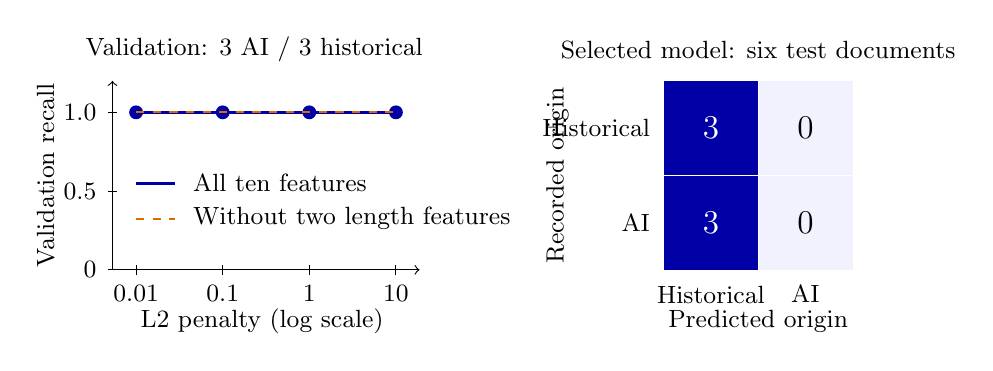
\begin{tikzpicture}[x=1cm,y=1cm,font=\small]
\node at (1.8,2.8) {Validation: 3 AI / 3 historical};
\draw[->] (0,0) -- (3.9,0);
\draw[->] (0,0) -- (0,2.4);
\foreach \height/\ticklabel in {0/0,1/0.5,2/1.0} {
  \draw (-0.06,\height) -- (0.06,\height);
  \node[left] at (-0.08,\height) {\ticklabel};
}
\foreach \position/\ticklabel in {0.3/0.01,1.4/0.1,2.5/1,3.6/10} {
  \draw (\position,-0.06) -- (\position,0.06);
  \node[below] at (\position,-0.08) {\ticklabel};
  \fill[blue!65!black] (\position,2) circle (2.5pt);
}
\draw[blue!65!black,very thick] (0.3,2) -- (3.6,2);
\draw[orange!85!black,thick,dashed] (0.3,2) -- (3.6,2);
\node[rotate=90] at (-0.85,1.2) {Validation recall};
\node at (1.9,-0.65) {L2 penalty (log scale)};
\draw[blue!65!black,very thick] (0.3,1.1) -- (0.8,1.1);
\node[right] at (0.9,1.1) {All ten features};
\draw[orange!85!black,thick,dashed] (0.3,0.65) -- (0.8,0.65);
\node[right] at (0.9,0.65) {Without two length features};
\node at (8.2,2.8) {Selected model: six test documents};
\fill[blue!65!black] (7,0) rectangle (8.2,2.4);
\fill[blue!5] (8.2,0) rectangle (9.4,2.4);
\draw[white] (7,1.2) -- (9.4,1.2);
\draw[white] (8.2,0) -- (8.2,2.4);
\node[text=white,font=\large] at (7.6,1.8) {3};
\node[text=white,font=\large] at (7.6,0.6) {3};
\node[font=\large] at (8.8,1.8) {0};
\node[font=\large] at (8.8,0.6) {0};
\node[left] at (6.95,1.8) {Historical};
\node[left] at (6.95,0.6) {AI};
\node[rotate=90] at (5.65,1.2) {Recorded origin};
\node[below] at (7.6,-0.08) {Historical};
\node[below] at (8.8,-0.08) {AI};
\node at (8.2,-0.65) {Predicted origin};
\end{tikzpicture}%
}
\caption{Validation success does not ensure useful test decisions. All eight
settings detect the three generated validation articles, whereas the selected
model misses all three generated test articles at its frozen threshold.}
\end{figure}

The absence of false positives is also weak evidence with only three
historical test articles. Even under an idealized independent Bernoulli model,
zero errors in three trials has a one-sided 95\% upper bound of
$1-0.05^{1/3}\approx0.632$ for the error probability. Shared publication and
generation conditions make independence questionable, so this is an
illustration of the sample-size problem, not a population-level confidence
claim. It cannot support a deployment guarantee of 5\% FPR.

The per-document explanations offer a further caution. In the held-out
historical passage on balanced valves, repeated trigrams contribute roughly
$-0.823$ to the selected model's logit, lowering its AI score. This is an
observation about these fitted weights, not a general rule about mechanical
writing or generation. In particular, it contradicts the tempting assumption
that any repetition feature must push a detector toward ``AI.''

\subsection{What the completed experiment must report}
The completed full study must report per-classifier AUROC, precision, recall,
F1, accuracy, and false-positive rate on untouched test data, together with
confusion counts for the joint screen. The code exports these point estimates
when supplied with valid data. Undefined precision, including the case where
nothing is flagged, is stored as JSON \texttt{null}. Validation scores remain
threshold-selection diagnostics, not unbiased performance estimates.

Compare the baseline with an always-negative screen, the authorship-only
classifier, the quality-only classifier, and a stronger documented detector
evaluated on the same held-out provenance examples. Use RAID as an additional
origin-detection stress test, not as a ready-made slop benchmark: origin labels
alone do not supply this project's quality annotations \cite{raid}. Add
ablation experiments removing repetition, length, and surface-marker features
in turn. Report subgroup false-positive rates by genre, text length, and
consented language-background metadata, together with sample counts and
intervals. Do not infer an author's language background from stylistic features.

A balanced detector dataset is useful for learning but does not reproduce web
prevalence. To illustrate why deployment precision matters, suppose---purely
hypothetically---that true prevalence is 5\%, sensitivity is 80\%, and FPR is
5\%. Among 1,000 documents, expected true positives are 40 and false positives
are 47.5, giving precision $40/(40+47.5)\approx45.7\%$. This arithmetic example
is not an experimental result. Confidence intervals and prevalence-aware
evaluation are needed before operational use.

\section{Second Development Cycle: Diagnostics and Readiness}
\subsection{Scope and separation of evidence}
All 24 pilot documents are now development material, including the six articles
used for the original final assessment. Their original results remain in the
record. No new untouched evaluation set has been constituted, and no contemporary
corpus with independent quality annotations has been acquired. Reusing an old
test set for diagnosis is legitimate once its role changes; calling the resulting
analysis another held-out success is not.

The second cycle adds two complementary development analyses and an implemented,
gated workflow for later independent annotation, calibration, model freezing and
evaluation. The authoritative prospective specification is
\texttt{cycle2/protocol.json}, with \texttt{cycle2/rubric.md} and the JSON bundle
and custody templates. Earlier CSV-schema drafts are explicitly superseded.
The separate \texttt{cycle2/exploratory\_plan.json} defines the supplementary
repeated-split experiment, not a competing final-evaluation protocol. A local
snapshot records the methodological hashes; it is not external preregistration,
an independent annotation audit, or a frozen trained model.

Public resources were reviewed for possible use. RAID offers authorship stress
tests, M4 addresses domain and generator variation, CoAuthor records mixed
human--AI writing, and SummEval supplies expert and crowd judgments of generated
summaries \cite{raid,m4,coauthor,summeval}. The review did not establish that any
provided the required combination of contemporary human provenance, this study's
quality rubric and a representative sampling frame. Existing summarization
ratings cannot simply be renamed as ground truth for a different construct.
Source details and permission gaps are recorded in
\texttt{cycle2/source\_audit.md}; no benchmark text was imported as qualified
primary data.

Bulk-access attempts through the terminal returned proxy 403 errors. Browser
access to documentation succeeded, but no external annotation file was analyzed.
This is an access limitation, not proof that suitable data do not exist.
Neither consent nor independent human judgment can be supplied by the assistant
on behalf of absent participants. The current annotation audit therefore has
zero documents and null agreement statistics. Final, independent-challenge,
prevalence and annual-trend results remain unavailable.

\subsection{Exploratory failure analysis and controls}
The first analysis uses leave-one-topic-pair-out assessment. In each of 12 folds,
one pair is assessed, three pairs select a cutoff, and the remaining eight
pairs fit the model. Normalization uses fitting data only. The original
configuration gives FNR 0.25, while the pilot-selected configuration gives FNR
approximately 0.333; both give FPR 0 on these reassigned development articles.
Their mean within-fold AUROC is 1.0. Scores from different fitted models are
not pooled into a global AUROC.

\begin{table}[htbp]
\centering\small
\begin{tabular}{lrrrr}
\toprule
Configuration & FPR & FNR & Accuracy & Mean fold AUROC \\
\midrule
Original & 0.000 & 0.250 & 0.875 & 1.000 \\
Pilot selected & 0.000 & 0.333 & 0.833 & 1.000 \\
Length only & 0.167 & 0.667 & 0.583 & 0.833 \\
Without repetition & 0.000 & 0.250 & 0.875 & 1.000 \\
\bottomrule
\end{tabular}
\caption{Exploratory leave-one-topic-pair-out development results on all 24 original pilot articles. These are not new final-test estimates.}
\end{table}

The supplementary analysis uses 100 seed-fixed 6/3/3 topic-pair partitions.
Each allocates six pairs to fitting, three to cutoff calibration and three
to assessment. Five settings are fitted: the original ten-feature model at
penalty 0.1; the selected eight-feature pilot setting at penalty 10; length-only
and repetition-only controls at penalty 0.1; and the ten-feature model without
its repetition features, also at penalty 0.1. The 500 fits are supplemented by
100 within-pair label-permutation fits on the original split. These are 600
calculations on 24 documents, not 600 independent experiments.

Three cutoff rules are compared: the original rule with conservative
tie-breaking; a cutoff immediately above the highest calibration-negative
score; and the midpoint between that maximum and the lowest positive score
when the calibration classes separate. The midpoint falls back to the original
rule otherwise. These comparisons are explicitly exploratory and do not replace
the original test record or select a new confirmatory model.

The original failure reproduces exactly in both analyses. For the selected
pilot model, the negative-maximum counterfactual uses a cutoff near 0.4603.
It recovers all three generated former-test positives but also flags one
historical article. A midpoint near 0.5002 separates those six documents.
The latter is not a new accuracy result: those documents are now development
material, and the question is how the decision rule behaves.

\begin{table}[htbp]
\centering\small
\begin{tabular}{llrrrr}
\toprule
Features & Cutoff rule & Mean FPR & Mean FNR & Median AUROC & Recall interval \\
\midrule
All ten & Legacy & 0.000 & 0.220 & 1.000 & [0.33, 1.00] \\
All ten & Negative max & 0.230 & 0.000 & 1.000 & [1.00, 1.00] \\
All ten & Midpoint & 0.010 & 0.000 & 1.000 & [1.00, 1.00] \\
Pilot selected & Legacy & 0.000 & 0.240 & 1.000 & [0.16, 1.00] \\
Pilot selected & Negative max & 0.260 & 0.000 & 1.000 & [1.00, 1.00] \\
Pilot selected & Midpoint & 0.040 & 0.007 & 1.000 & [1.00, 1.00] \\
Length only & Legacy & 0.087 & 0.657 & 1.000 & [0.00, 1.00] \\
Length only & Negative max & 0.240 & 0.390 & 1.000 & [0.00, 1.00] \\
Length only & Midpoint & 0.153 & 0.500 & 1.000 & [0.00, 1.00] \\
Repetition only & Legacy & 0.120 & 0.720 & 0.833 & [0.00, 1.00] \\
Repetition only & Negative max & 0.153 & 0.720 & 0.833 & [0.00, 1.00] \\
Repetition only & Midpoint & 0.120 & 0.720 & 0.833 & [0.00, 1.00] \\
No repetition & Legacy & 0.000 & 0.210 & 1.000 & [0.33, 1.00] \\
No repetition & Negative max & 0.223 & 0.000 & 1.000 & [1.00, 1.00] \\
No repetition & Midpoint & 0.003 & 0.000 & 1.000 & [1.00, 1.00] \\
\bottomrule
\end{tabular}
\caption{Exploratory cycle-two diagnostics over 100 repeated topic-pair splits of the same 24 pilot documents. Intervals are the 2.5th and 97.5th percentiles across splits, not confidence intervals for modern-web performance.}
\end{table}

Across the 100 supplementary partitions, the selected pilot setting with the
legacy rule has mean FNR 0.240 and mean FPR 0.000. The negative-maximum rule
reduces mean FNR to 0.000 but raises mean FPR to 0.260. The midpoint gives mean
FNR approximately 0.007 and FPR 0.040. This is an operating-point trade-off
within the pilot, not established deployment performance. The length-only
control reaches median assessment AUROC 1.0 despite legacy-threshold mean FNR
approximately 0.657. Simple surface differences can therefore account for much
of the ranking in these tiny assessment sets without producing reliable
decisions or establishing an authorship mechanism.

The two permutation procedures answer different diagnostic questions. The
99-permutation leave-pair-out procedure gives a Monte Carlo value of 0.01 for
mean within-fold AUROC. The supplementary 100-permutation procedure, using
the original six-document assessment split, gives a tail fraction near 0.099.
Their assessment statistics and training allocations differ; the values must
not be selected according to which appears more favorable. Both concern
association under within-pair exchangeability, not proof that origin rather
than source, era or register caused that association.

On the frozen selected pilot model, whitespace changes and uppercase conversion
leave all 24 scores unchanged. Prefixing each sentence with a hyphen changes
four generated-positive decisions to unflagged, with a maximum absolute score
change near 0.01849. This adds formatting without adding substantive claims.
Replacing digit sequences with the word ``number'' changes some scores but
no flags; because that manipulation changes content, it is a destructive
sensitivity probe rather than a meaning-preserving robustness test.

The immediate failure mechanism is identifiable: the selected operating point
does not transfer to the assessment score range even when ranking is preserved.
Its underlying causes cannot be separated here. Historical era, publication
source, register and the generating assistant are confounded with origin.
Source-disjoint performance is \emph{not identifiable}; independent translation,
proficiency and mixed-authorship challenge results are \emph{not available}.
Repeated splitting cannot create missing source diversity.

\subsection{Uncertainty and prospective methodology}
Supplementary split percentiles describe sensitivity conditional on the same
24 documents, not confidence intervals for modern-web performance. The
leave-pair-out analysis additionally reports topic-cluster bootstrap intervals
conditional on fitted predictions, excluding training uncertainty. A bootstrap
that contains only zero errors is not evidence of zero population risk.
Exact binomial intervals are separately labeled as requiring independence,
which shared sources violate. Repeated assessments must not be counted as
new independent observations.

The authoritative prospective protocol covers English public-web-style text
created from January 1, 2024 through September 10, 2026, with consented or
reuse-permitted origin evidence. Its collection targets and minimum evaluation
strata are recorded as plans, not achieved counts or a completed power analysis.
Genre, topic, proficiency, formatting, authorship pattern and generator-family
metadata are required, with unknown metadata identified rather than inferred.
A stratified curated benchmark is not an internet probability sample.

The confirmatory comparison fixes the original ten-feature model at L2 penalty
0.1. Independent development and calibration bundles must pass annotation,
provenance, rights and privacy admission and remain source-, author- and
cluster-disjoint. The model is fitted before inspecting calibration scores.
One negative representative per cluster is selected by document ID, not by its
score, and each head requires at least 120 negative calibration clusters under
the protocol.

The implemented calibration rule selects a negative-score order statistic,
following the independent-negative principle of Neyman--Pearson calibration
\cite{tong2018}. For $n$ independent exchangeable negative scores, target FPR
$\alpha$, and rank $k$ in ascending order, the violation bound is
\begin{equation}
 B(n,k,\alpha)=\sum_{j=k}^{n}\binom{n}{j}
                  (1-\alpha)^j\alpha^{n-j}.
\end{equation}
The smallest rank with $B(n,k,\alpha)\leq\delta$ is used, and the cutoff is
the next representable value above that score. Here $\alpha=0.05$ and
$\delta=0.025$ per head. The theoretical minimum is 72 independent negatives;
the protocol's minimum of 120 is stricter. Many passages from one publisher
are not many independent calibration sources.

These assumptions must be justified through collection and review. The
two per-head tolerances concern marginal error control under exchangeability;
they do not establish a 5\% FPR for the combined slop screen or protect against
distribution shift. The workflow reports joint-screen performance separately
and does not infer reliability from an apparently favorable aggregate score.

\subsection{Annotation, custody, and release status}
The authoritative rubric retains the three quality dimensions and critical-error
rule. Two fixed, distinct, independent human raters work blind to origin and
detector output; a third human resolves decision disagreements. Initial
judgments are preserved. Admission requires at least 100 paired documents,
raw agreement at least 0.80, a lower 95\% cluster-bootstrap kappa bound at
least 0.60, and at least 95\% resolved quality labels. These are design choices,
not universal validity standards. The audit reports binary Cohen's kappa,
dimension-level quadratically weighted kappa, uncertainty and adjudication
counts, and defined bootstrap-replicate counts. Constant-label kappa remains
undefined.

The actual audit has no independent ratings and therefore no observed agreement
statistic. Artificial software fixtures test arithmetic and workflow behavior;
they are not a human annotation study. Likewise, Boolean metadata claiming
consent or independence are not proof of either. A responsible investigator
must verify the underlying evidence.

The implemented workflow can fit and calibrate admitted bundles, record
method/data/model hashes, freeze a model against an independent custodian's
commitment, and evaluate the committed final bundle without changing thresholds.
It checks source/author separation, final-cell counts, topic/source/generator
coverage and required challenge conditions. Mixed or unknown origin does not
become a human label; short or unresolved cases remain visible in coverage.
Per-condition and subgroup FPR, FNR and other metrics are accompanied by
uncertainty and small-cell cautions.

None of those confirmatory steps has been completed on a qualifying real corpus.
The template audit is blocked, there is no trained confirmatory model or
independently held final set, and no final or independent-challenge result is
reported. A local method snapshot is not the later model freeze. Error-adjusted
prevalence remains unavailable without a separate probability sample and
independently audited, transportable joint-screen error rates; annual trends
also require comparable frames and time-specific audits. The package now
contains executable development evidence and guarded prospective machinery,
not a completed validation or a guarantee of publication suitability.

\section{Limitations, Ethics, and Next Steps}
The main limitation remains the absence of a representative corpus with
independently adjudicated quality labels. A working optimizer does not show
that its features can recognize authorship or poor quality across the web.
It may instead learn genre, translation patterns, author proficiency, or
formatting. A low empirical FPR on one validation set likewise offers no
guarantee of fair or accurate behavior elsewhere, as existing detector audits
make clear \cite{liang,tufts}.

The pilot adds an observed failure to these design concerns. Its conservative
threshold does not transfer even across a handful of topic-disjoint articles
from a tightly controlled source setting. The appropriate response is a
new development cycle, not retrospective threshold adjustment presented as
held-out success. That cycle has now completed exploratory diagnostics on
the reassigned pilot articles and locally frozen its prospective rubric,
sampling design and calibration rule. It has not obtained contemporary
provenance-controlled human text, independent quality labels, or an untouched
final set. Source-disjoint validation and confirmatory scoring remain pending;
their absence is a limit on the conclusions, not a missing number to infer.

Outputs are for manual review, not automatic removal, accusations against
students or authors, or public labeling of individuals. Collection should
use permitted public material or consented writing, minimize personal
information, and record reuse permissions before any text is released.
Aggregate findings and documentation are preferable to unnecessary author
identifiers. AI assistance in preparing the draft and generated examples
must be disclosed according to the eventual venue's requirements. For
transparency, this draft was prepared and revised with an AI assistant, which
also authored the pilot's generated articles.

The full study now has a locally frozen rubric and sampling protocol, but
still needs provenance-controlled collection, an independent annotation-agreement
audit, a qualified model freeze, and evaluation on untouched and challenge sets.
Only after those steps can error-adjusted
prevalence and annual trends be estimated responsibly. A publishable
contribution would rest on the transparency and adequacy of that evidence,
not on securing a particular conclusion in advance.

\section{Conclusion}
The project separates a broad concern into two measurable tasks: estimating
low-quality machine-generated web text and evaluating a detector for it.
Existing evidence motivates both without establishing an internet-wide slop
majority \cite{pew,pewmethods,dolezal}. The implementation makes the detector
inspectable, while the pilot shows why inspection must extend beyond a
favorable aggregate metric: perfect ranking coexists with zero detection at
the chosen threshold. Adequate modern-web performance and a takeover of the
specified web population remain open empirical questions. The study is
stronger for leaving them open than it would be for answering them by design.
The second cycle adds reproducible evidence of threshold sensitivity and
formatting dependence, while showing why the available corpus cannot separate
source and era from authorship. The package is not yet a completed empirical
validation or a guarantee of publication suitability.

\appendix
\section{Reproducing the Implementation}
The companion \texttt{README.md} specifies CSV preparation and remaining
research work. Once a real, audited corpus has been prepared, run:
\begin{lstlisting}
python detector.py train corpus.csv model.json results.json
python detector.py predict model.json article.txt
\end{lstlisting}
The first command fits both classifiers and saves their coefficients,
normalization constants, thresholds, and dataset fingerprint. The second
extracts the same features from an English text file and emits scores,
contributions, and a review flag. No fitted two-head model or completed
quality-annotated web corpus is bundled. The separate authorship pilot includes
its source passages, generated text, fitted weights, selection ledger, and
per-document results. To reproduce its three stages in a fresh output
directory, run:
\begin{lstlisting}
python run_pilot.py prepare --output pilot/reproduction
python run_pilot.py select --output pilot/reproduction
python run_pilot.py evaluate --output pilot/reproduction
\end{lstlisting}
These commands replay a fixed experiment; they do not produce independent
new generations or a new benchmark. The random seed reproduces style
assignment only. \texttt{pilot/artifacts} contains the recorded run used in
this paper. A supplied text file can be scored with the selected pilot model:
\begin{lstlisting}
python detector.py predict pilot/artifacts/selected_model.json article.txt
\end{lstlisting}
The second-cycle development diagnostics and readiness audit run separately:
\begin{lstlisting}
python research_cycle.py diagnose
python research_cycle.py snapshot
python cycle2_workflow.py audit cycle2/bundle_template.json cycle2/artifacts/annotation_audit.json
\end{lstlisting}
The template audit intentionally exits with an error because independent
data and review are missing. \texttt{cycle2/README.md} distinguishes
implemented diagnostics and the gated prospective workflow from completed
empirical evaluation. Its bundle and annotation templates are empty; they
are not a collected dataset.
The methodological freeze records hashes locally and is not an externally
timestamped registration. Build this document with:
\begin{lstlisting}
latexmk -pdf -interaction=nonstopmode -halt-on-error main.tex
\end{lstlisting}

\begin{thebibliography}{99}
\bibitem{pew}
S. Bestvater, A. Smith, C. TerBush, C. Baronavski, and J. Chavda.
\emph{How Much of the Internet Is Written With AI?}
Pew Research Center, August 20, 2026.

\bibitem{pewmethods}
S. Bestvater, A. Smith, C. TerBush, C. Baronavski, and J. Chavda.
\emph{Methodology: How Much of the Internet Is Written With AI?}
Pew Research Center, August 20, 2026.

\bibitem{dolezal}
J. Dolezal, S. Alam, M. Graham, and M. Bohacek.
\emph{The Impact of AI-Generated Text on the Internet}.
arXiv:2604.26965, version 1, April 14, 2026. Preprint.

\bibitem{raid}
L. Dugan, A. Hwang, F. Trhl\'{i}k, A. Zhu, J. M. Ludan, H. Xu,
D. Ippolito, and C. Callison-Burch.
RAID: A Shared Benchmark for Robust Evaluation of Machine-Generated Text
Detectors. \emph{Proceedings of ACL}, 2024.
doi:10.18653/v1/2024.acl-long.674.

\bibitem{tufts}
B. Tufts, X. Zhao, and L. Li.
A Practical Examination of AI-Generated Text Detectors for Large Language
Models. \emph{Findings of NAACL}, pp. 4839--4856, 2025.
doi:10.18653/v1/2025.findings-naacl.271.

\bibitem{liang}
W. Liang, M. Yuksekgonul, Y. Mao, E. Wu, and J. Zou.
GPT detectors are biased against non-native English writers.
\emph{Patterns}, 4(7):100779, 2023.
doi:10.1016/j.patter.2023.100779.

\bibitem{tong2018}
X. Tong, Y. Feng, and J. J. Li.
Neyman-Pearson classification algorithms and NP receiver operating characteristics.
\emph{Science Advances}, 4(2):eaao1659, 2018.
doi:10.1126/sciadv.aao1659.

\bibitem{m4}
Y. Wang et al.
M4: Multi-generator, Multi-domain, and Multi-lingual Black-Box Machine-Generated
Text Detection. \emph{Proceedings of EACL}, pp. 1369--1407, 2024.
doi:10.18653/v1/2024.eacl-long.83.

\bibitem{coauthor}
M. Lee, P. Liang, and Q. Yang.
CoAuthor: Designing a Human-AI Collaborative Writing Dataset for Exploring
Language Model Capabilities. \emph{Proceedings of CHI}, 2022.
doi:10.1145/3491102.3502030.

\bibitem{summeval}
A. R. Fabbri, W. Kry\'{s}ci\'{n}ski, B. McCann, C. Xiong, R. Socher, and D. Radev.
SummEval: Re-evaluating Summarization Evaluation.
\emph{Transactions of the Association for Computational Linguistics}, 9:391--409,
2021. doi:10.1162/tacl\_a\_00373.
\end{thebibliography}
\end{document}